\documentclass[main.tex]{subfiles} % Subfile-Class

%==============================================================================%
%                                   Subfile                                    %
%==============================================================================%

\begin{document}

% Template

\section{Linienfolger - Reglerauslegung und Parametrierung}~\label{apdx:LineFollowerRegler}

\subsection*{Sensor Funktionsweise}~\label{apdx:Liniensensor_auswertung}

Der Liniensensor wurde, wie bereits in PREN1 ausführlich dokumentiert, mit acht
Helligkeitssensoren realisiert. Die Idee ist, dass diese Sensoren, die im
sichtbaren Lichtspektrum empfindlich sind, die Reflexion des Klebebandes
auswerten. Da das Klebeband mit UV-Licht bestrahlt wird, fluoresziert es stark
und bildet einen deutlichen Kontrast zur Bodenfuge bzw. zu den Fliesen des
Wettkampfbodens.

% TODO: Abbildung

Der Vorwiderstand der Messzellen ist so dimensioniert, dass der
lichtempfindliche Transistor in Sättigung geht, sobald sich eine Linie
unterhalb des Sensors befindet. Dadurch wird der starke Kontrast auch in der
Spannung über der Messzelle deutlich sichtbar.

\subsection*{Sensor Auswertung}

\paragraph{Auslesen und normieren der Werte}

Der Sensor wird analog über einen A/D-Wandler ausgelesen. Die acht Messwerte
werden in einem Array gespeichert.

Anschliessend werden alle Messwerte auf einen Bereich zwischen $0 \ddots 1000$
normiert. Dazu sind Kalibrationswerte für die Maximal- und Minimalspannungen
($Calib_{\max}$ und $Calib_{\min}$) erforderlich, welche für jede Zelle
individuell durch Messungen auf dem Wettkampfboden ermittelt wurden.

\[
    Val_{norm} = (Val_{raw} - Calib_{\min}) \cdot \frac{1000}{Calib_{\max} - Calib_{\min}}
\]

\paragraph{Gewichtetes Summieren der Werte}
Ziel ist es, die Linienposition in Form einer einzelnen Zahl auszugeben. Dazu
werden die normierten Sensorwerte herangezogen, und gewichtet zusammengezählt.

\[
    LinePos = \frac{0 \cdot Val_{norm}[0] + 1 \cdot Val_{norm}[1] + \cdots + 7 \cdot Val_{norm}[7]}{\sum_{k=0}^{7}(Val_{norm}[i])}
\]

Ergibt die Berechnung $0$ oder $8000$, so befindet sich die Linie am äusseren
Anschlag. Befindet sich die Linie in der Mitte, ergibt die Berechnung $3500$,
was auch der Sollwert des Linienfolgers ist.

\subsection*{Regler Aufbau}

\begin{figure}[H]
    \centering
    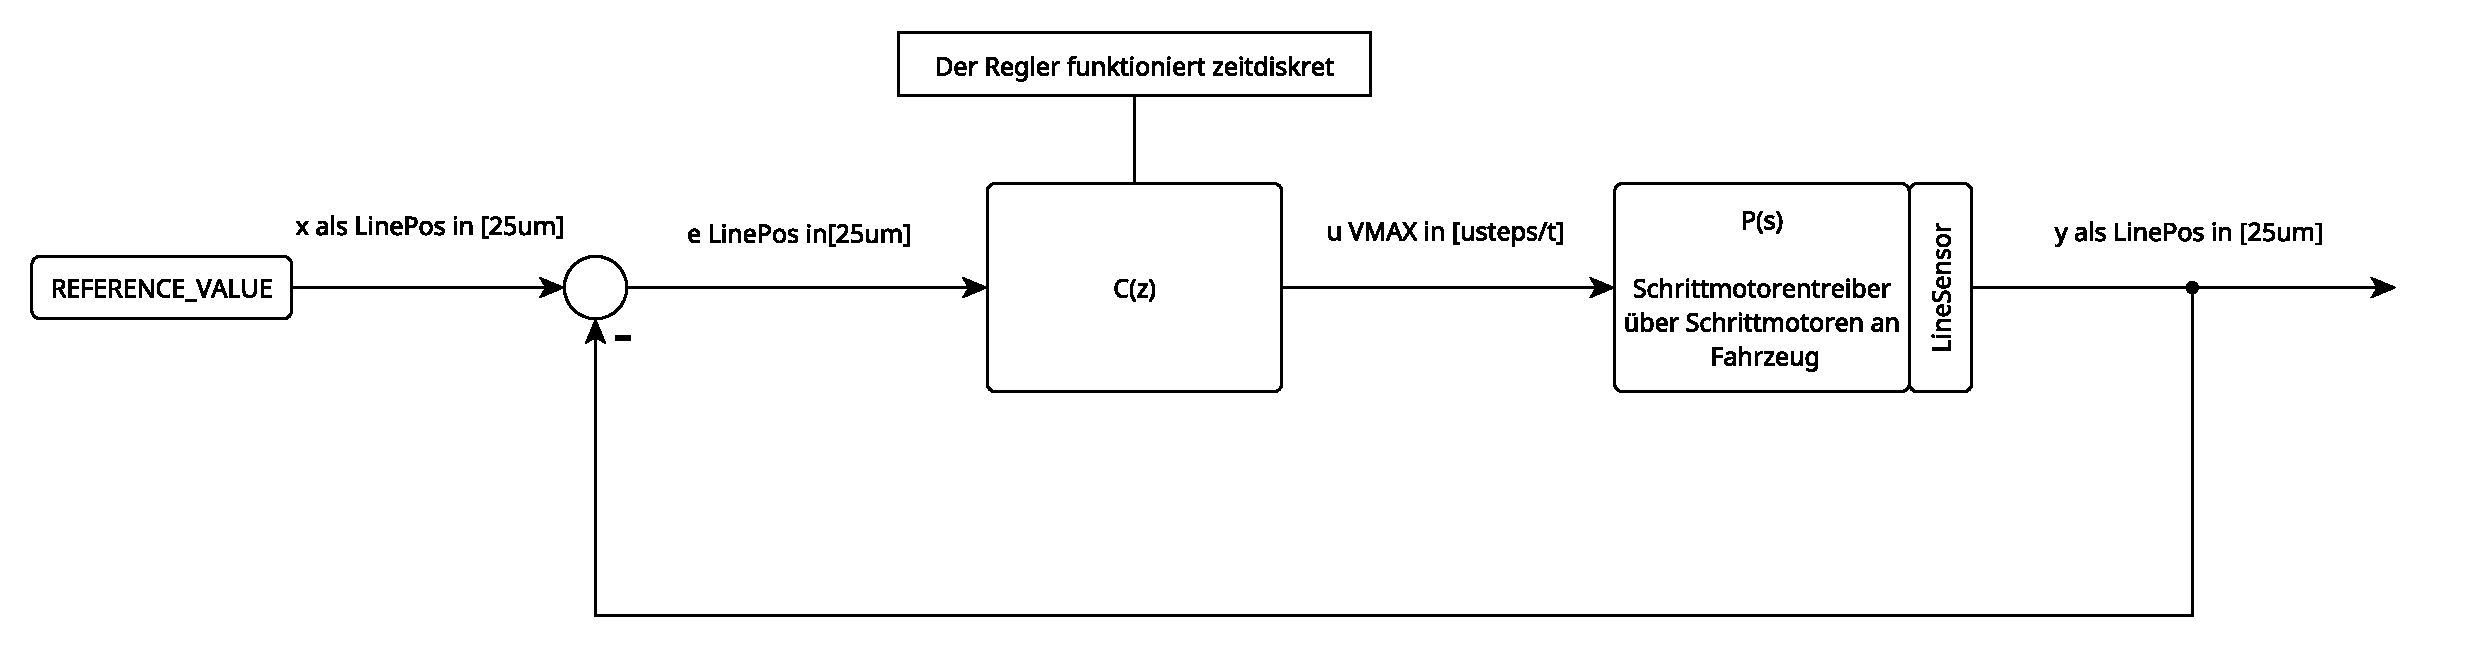
\includegraphics[width=1.0\linewidth]{fig_Parametrierung_Linienfolgeregler/RegelProzess_Linienfolger.pdf}
    \caption{Reglerprozess des Linienfolgers}~\label{fig:Linienfolger_RegelProzess}
\end{figure}

Die Abbildung~\ref{fig:Linienfolger_RegelProzess} zeigt schematisch, wie der
Regelprozess funktioniert. Eingangsgrösse ist die Bezugsgrösse $x$, die im
vorhergehenden Abschnitt auf konstante $3500$ festgelegt ist. Diese Grösse gibt
die auf den Messzellenabstand aufgelöste Linienposition auf einer Skala von $0
    \dots 8000$ an und hat die Einheit $25\mu m$.

Der zeitdiskrete Regler $C(z)$ implementiert einen zeitdiskreten PD-Regler,
dessen Parametrierung im folgenden Abschnitt \textit{Reglerparametrierung}
näher erläutert wird. Die Ausgangsgrösse $u$ des Reglers entspricht der
Motordrehzahl in $\frac{\mu \text{steps}}{t}$, die im Prozess $P(s)$ durch die
Motortreiber in eine Fahrbewegung umgesetzt wird.

Der Prozess $P(s)$ beschreibt das gesamte Verhalten des Fahrzeugs. Dies umfasst
den Regelkreis von der Ausgabe der Fahrsignale an die Motortreiber über das
gesamte Fahrverhalten bis hin zur erneuten Auswertung der Streckenlage über den
Liniensensor. Dementsprechend ist die Ausgangsgrösse dieses Prozesses $y$
wieder die Linienposition, die am Eingang des Reglers mit der Referenzgrösse
verglichen wird, um den Regelfehler $e$ zu bestimmen.

\subsection*{Regler Parametrierung}~\label{apdx:Regler_Parametrierung}

\subsubsection*{Aufzeichnung der Sprungantwort und Prozessmodellierung}

Um das Fahrverhalten zu analysieren, ist ein einfacher P-Regler implementiert.

\[
    C(z) = k_p \cdot e(z)
\]

Der Parameter $k_p = 5$ wurde so gewählt, dass das Fahrzeug Fahrfehler über
eine längere Strecke einigermassen kompensieren kann. Um eine Sprungantwort
aufzuzeichnen, wird dem Fahrzeug ein Sprung in Form eines Klebebandes
vorgesetzt und der Ausgang des Liniensensors via USB-CDC Schnittstelle
ausgegeben.

\begin{figure}[H]
    \centering
    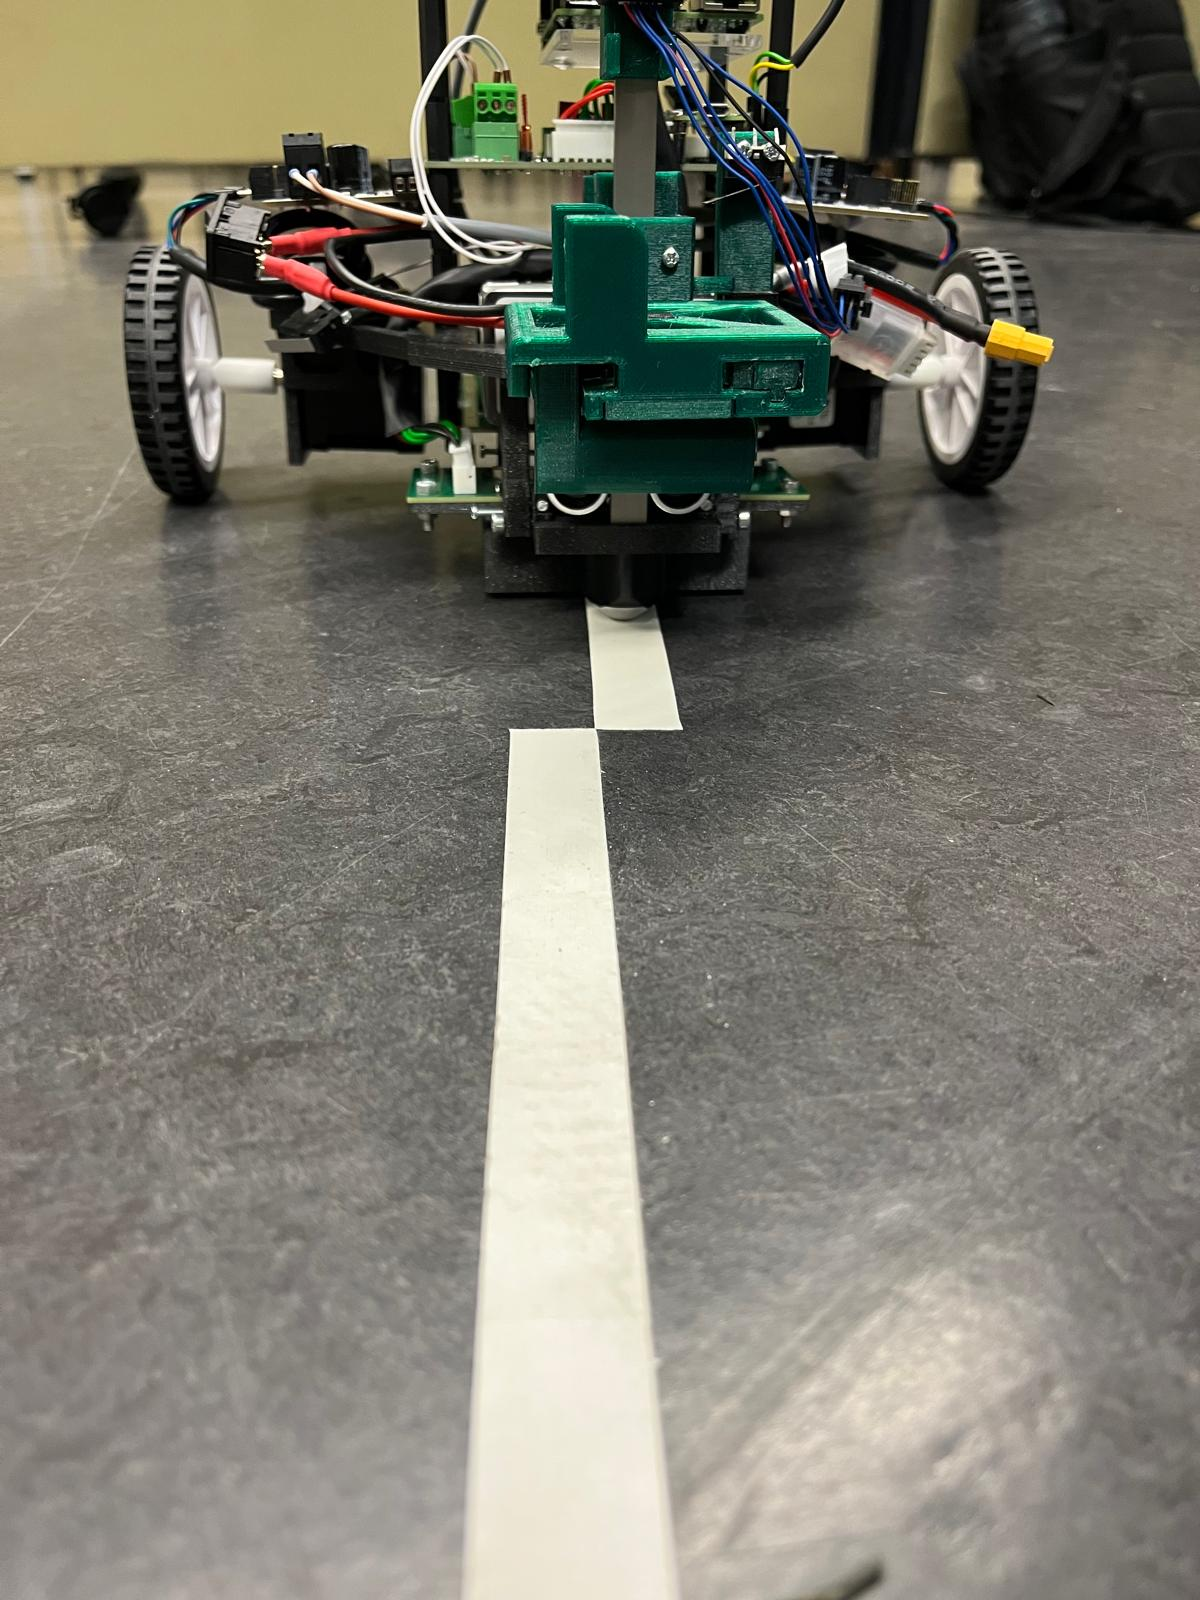
\includegraphics[width=0.5\linewidth]{fig_Parametrierung_Linienfolgeregler/Versuchsaufbau_Sprungantwort.jpeg}
    \caption{Versuchsaufbau zum Aufzeichnen der Sprungantwort}~\label{fig:Linienfolger_Versuchsaufbau_Sprungantwort}
\end{figure}

Abbildung~\ref{fig:Linienfolger_Versuchsaufbau_Sprungantwort} zeigt den
entsprechenden Versuchsaufbau. Mit Hilfe von Matlab kann nun das
Fahrzeugverhalten grafisch dargestellt werden.

Die gemessene Grösse des Liniensensors entspricht jedoch nicht direkt der
Sprungantwort selbst, sondern vielmehr der aktuellen Abweichung von dieser. Aus
dem Wert des Liniensensors kann somit der aktuelle Regelfehler $e[k]$ abgelesen
werden.

Wird dieser Fehler mit einem Referenzsignal verglichen, das einen Sprung von
der Mittelposition auf etwa $50mm$ beschreibt, lässt sich die tatsächliche
Sprungantwort ableiten.

\begin{figure}[H]
    \centering
    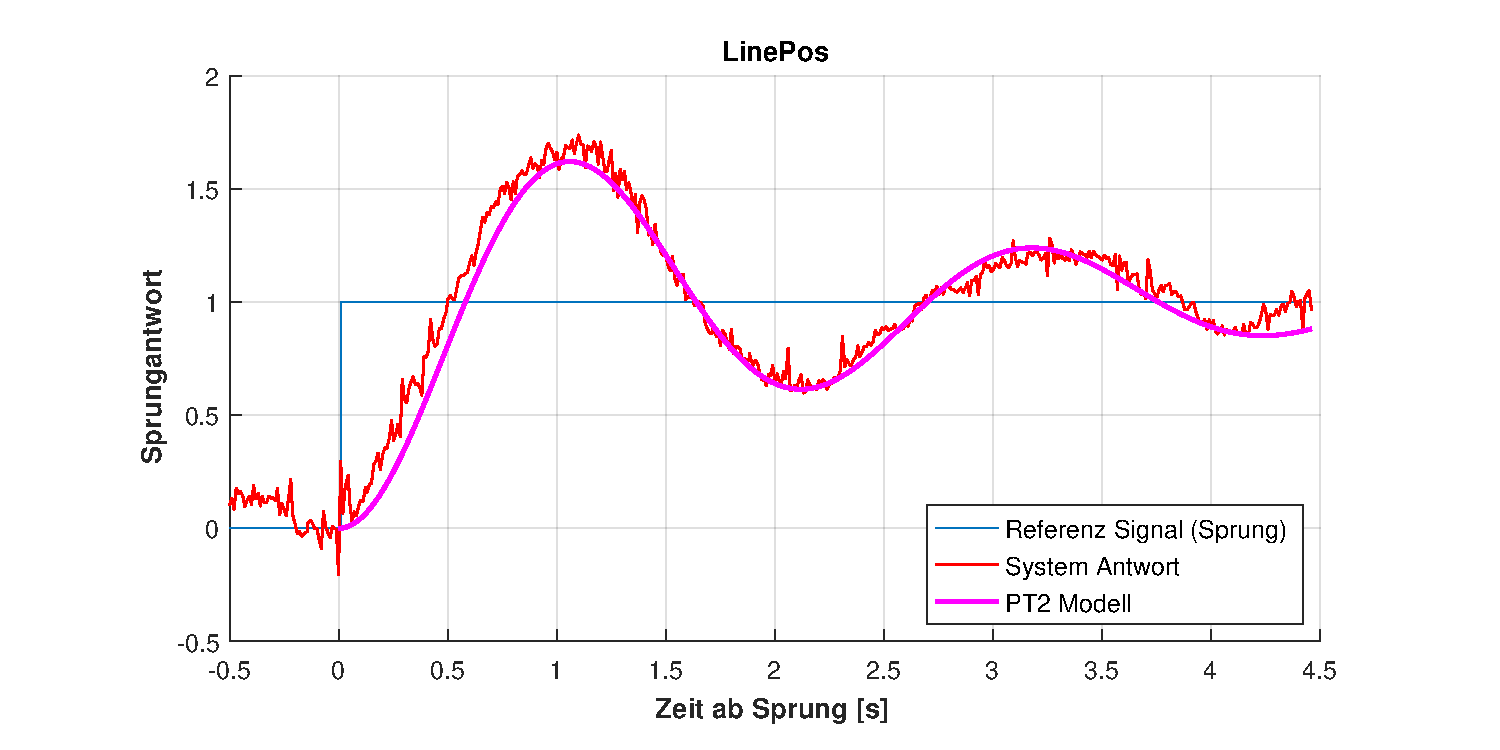
\includegraphics[width=0.5\linewidth]{fig_Parametrierung_Linienfolgeregler/Sprungantwort_System.pdf}
    \caption{Sprungantwort und PT2 Modell}~\label{fig:Sprungantwort}
\end{figure}

Abbildung~\ref{fig:Sprungantwort} zeigt das Ergebnis dieses Experiments. Die
rote Linie stellt die aufgezeichnete Sprungantwort dar, die magentafarbene
Linie das zugehörige PT2-Modell.

Die Sprungantwort zeigt, dass das System sehr direkt reagiert und praktisch
keine erkennbare Totzeit aufweist. Da dies jedoch in der Realität kaum möglich
ist, wurde dem PT2-Prozessmodell eine zusätzliche Totzeit von $20ms$
hinzugefügt, was etwa zwei Abtastraten entspricht.

Das gezeigte PT2 Modell besitzt die folgenden Parameter:

\begin{itemize}
    \item $kp = 1$
    \item $\omega = 3.0 rad$
    \item $\zeta = 0.15$
    \item $T_t = 0.02 s$
\end{itemize}

Daher, dass der Regler $C(z)$ mit seinem Verstärkungsfaktor $kp = 5$ bekannt
ist, lässt sich aus dieser Closed-Loop Systemantwort der Prozess $P(s)$
algebraisch ermitteln.

\[
    P(s) \approx \frac{G_{PT2}}{1 - G_{PT2}}
\]

Mit $G_{PT2}$, der Closed-Loop Systemantwort, dargestellt durch das PT2-Modell.

\subsubsection*{Auswertung und Auslegung des Reglers}

\begin{figure}[H]
    \centering
    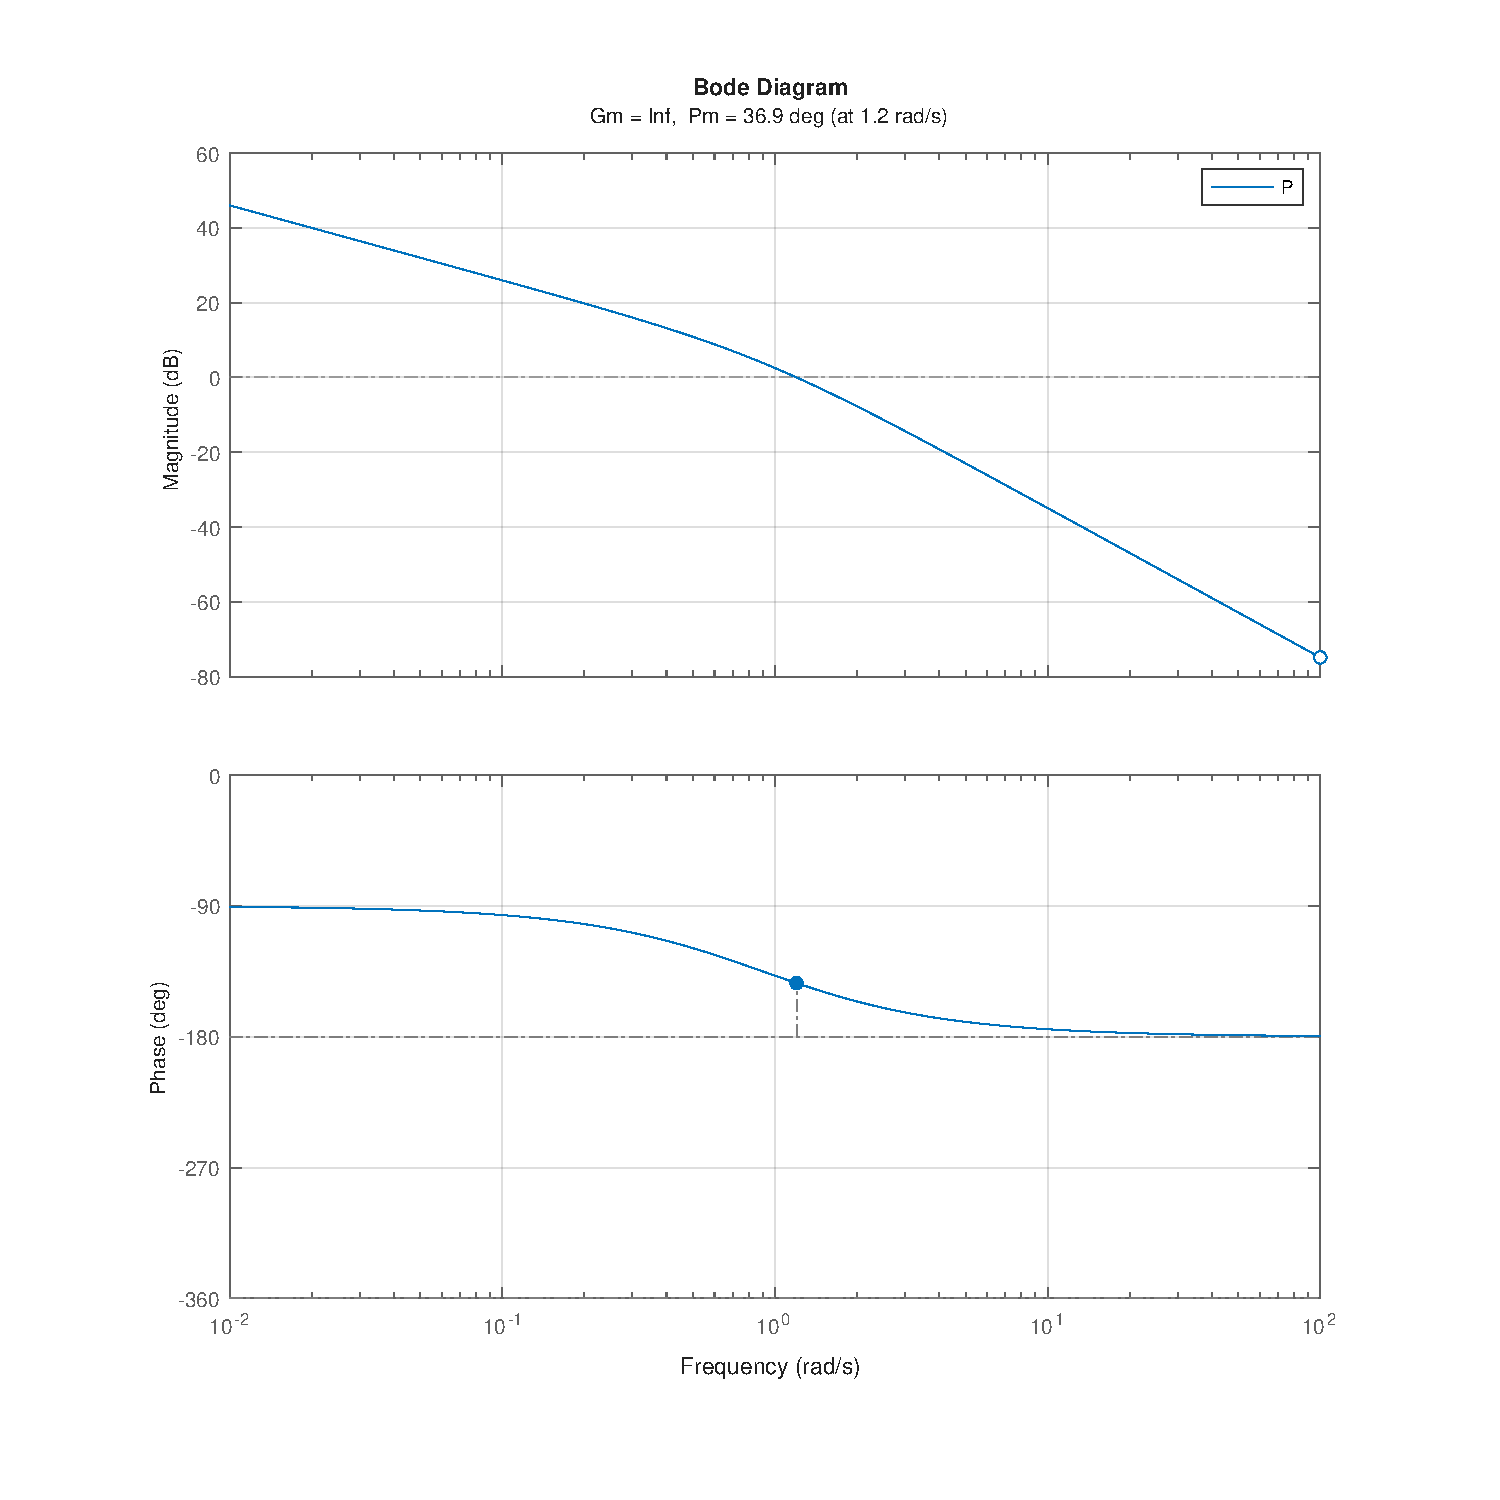
\includegraphics[width=0.5\linewidth]{fig_Parametrierung_Linienfolgeregler/Bode_Plot_Prozess.pdf}
    \caption{Bodeplot mit eingezeichnter Phasen- und Amplitudenreserve}~\label{fig:MarginPlot_raw}
\end{figure}

\begin{figure}[H]
    \centering
    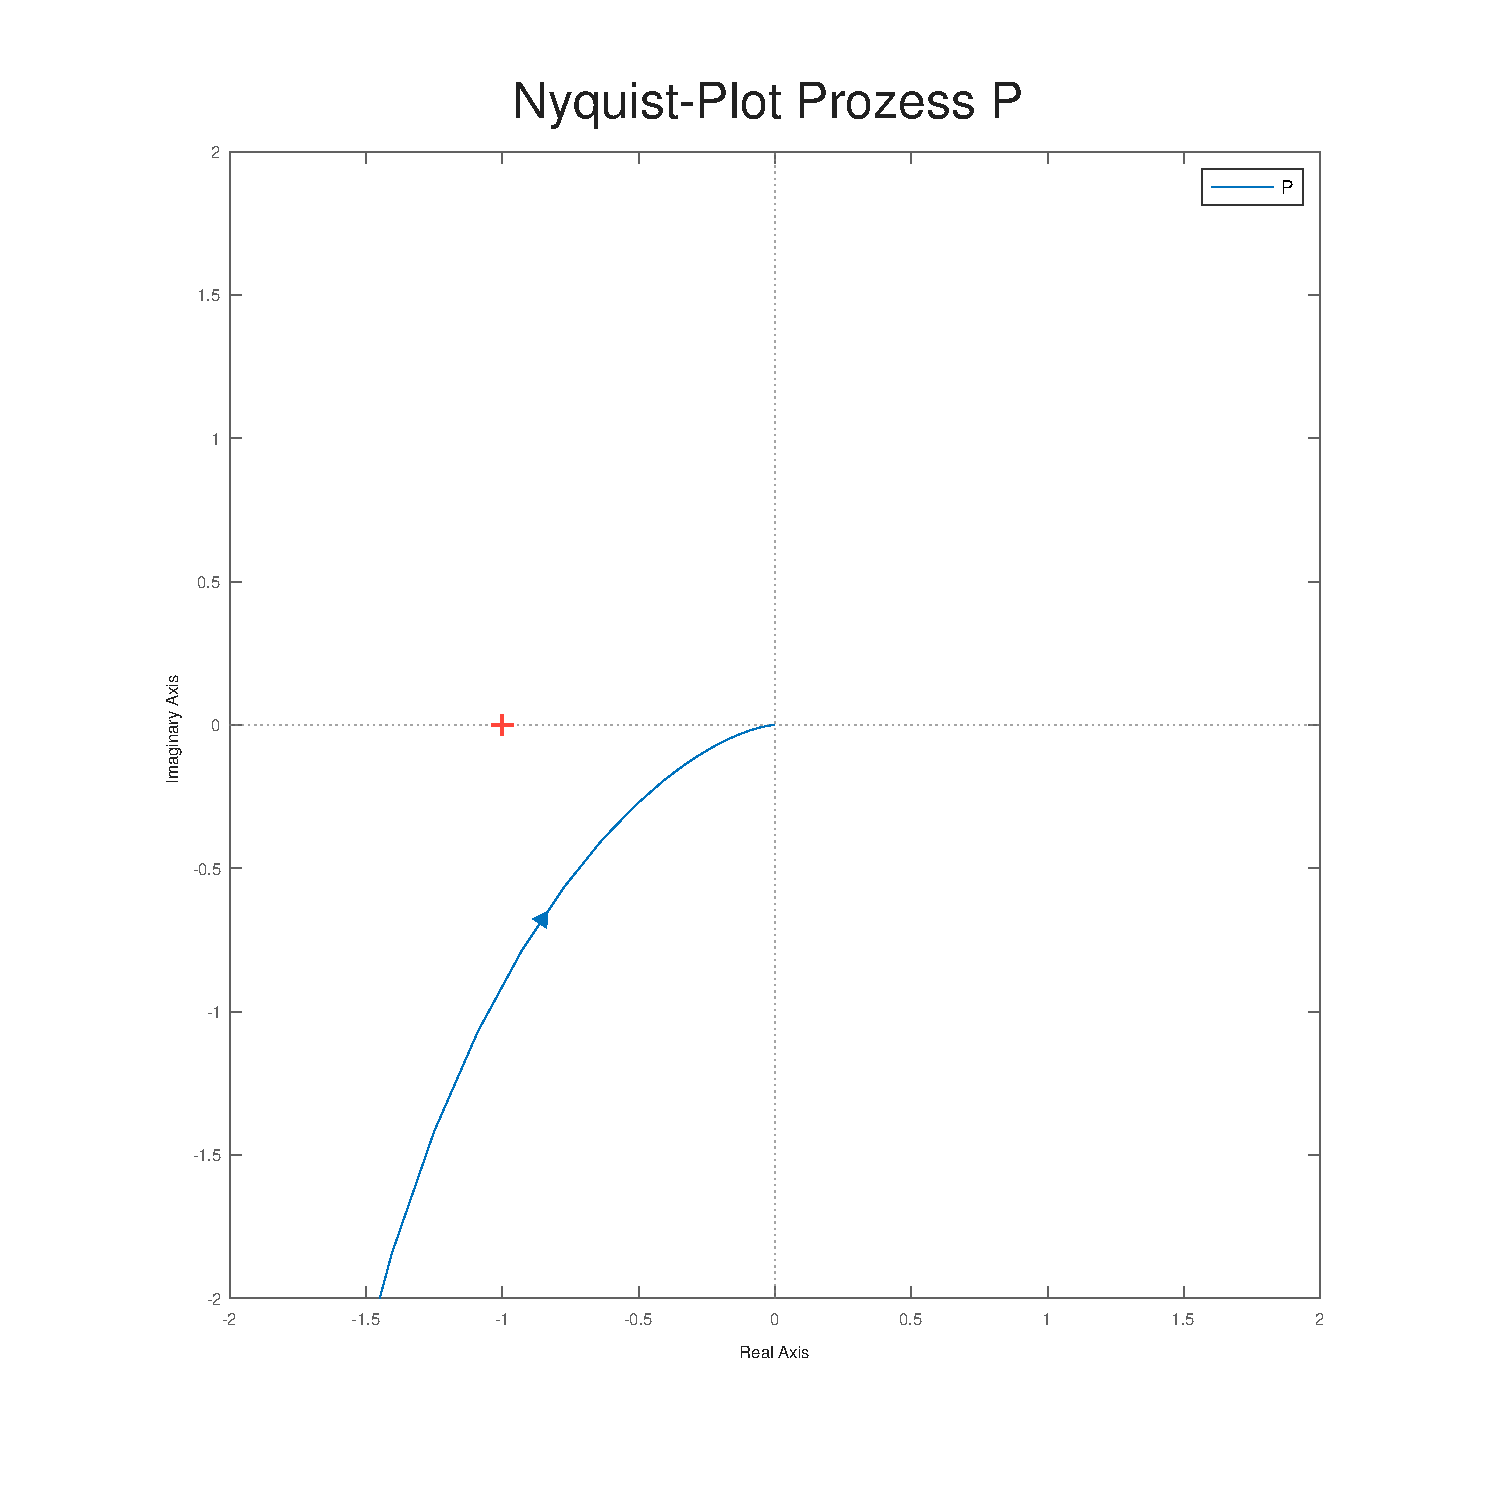
\includegraphics[width=0.5\linewidth]{fig_Parametrierung_Linienfolgeregler/NyquistPlot_System.pdf}
    \caption{Nyquistdiagramm des Prozesses $P(s)$}~\label{fig:Nyquist_raw}
\end{figure}

Abbildung~\ref{fig:MarginPlot_raw} zeigt den Bodeplot des Prozesses $P(s)$ mit
eingezeichneter Phasenreserve, während Abbildung~\ref{fig:Nyquist_raw} den
Nyquistplot des Systems zeigt.

\paragraph{Anforderungen an den Regler:} Das Einschwingverhalten des Prozesses sollte deutlich geglättet sein. Ein
einmaliges Überschwingen wird kaum vollständig zu vermeiden sein, jedoch sollte
der Regler innerhalb von $\approx 500 ms$ mindestens 90\% des Sprunges erreicht
haben. Damit ist der Regler in der Lage, das Fahrzeug innerhalb einer
\textit{minimalen Hindernisdistanz}, die in der FAQ mit 300mm angegeben ist,
mittig auf der Linie zu positionieren. Ein zwischenzeitliches Überschwingen von
20\% wird toleriert, da auf der Wettkampfstrecke in der Regel nicht mit
Sprüngen zu rechnen ist. Eine solche Regel sollte daher völlig ausreichen, um
einer Linie geradeaus zu folgen. Da eine exakte Kurvenfahrt nicht erforderlich
ist, ist ein verbleibender Regelfehler akzeptabel. Ein Integralanteil ist daher
nicht erforderlich.

\subsubsection*{Festlegung des Reglertyps und Parametrierung}

Die Abbildungen~\ref{fig:Nyquist_raw} und ~\ref{fig:MarginPlot_raw} zeigen,
dass der Prozess prinzipiell durch einen P-Regler mit der
Verstärkungskonstanten $k_p$ beschleunigt werden kann. Durch die zentrische
Streckung der Nyquist-Kurve nähert sich diese jedoch sehr schnell dem rot
markierten Punkt $-1$. Bei höheren Verstärkungen ist daher eine Phasenanhebung
erforderlich. Aus diesem Grund wurde ein PD-Regler gewählt. Wird der aktuell
verfügbare Verstärkungsspielraum voll ausgenutzt, so ergibt sich näherungsweise
ein Verstärkungsfaktor von $k_p = 32$. In diesem Fall geht die Nyquist-Kurve
jedoch nahe am Punkt $-1$ vorbei, wodurch das System schwingt und instabil
wird.

Mit dem D-Anteil des Reglers kann die Phase bis zu einer Frequenz von etwa $10
    \cdot \omega_{pc}$ in Richtung $+90^\circ$ verschoben werden, wodurch das
System wieder stabilisiert wird.

Der Eingesetzte Regler der Form
\[
    C(s) = k_p \cdot (1 + \frac{T_d \cdot s}{1 + \frac{T_d}{10} \cdot s})
\]

Mit den Parametern $kp = 32$, $Td = 0.08$ kann somit ein sehr stabiles System
erreicht werden. Der Phasen- und Amplitudenverlauf sowie das aktualisierte
Nyquist-Diagramm des geregelten Prozesses sind in
Abbildung~\ref{fig:MarginPlot_geregelt} und
Abbildung~\ref{fig:Nyquist_geregelt} dargestellt.

\begin{figure}[H]
    \centering
    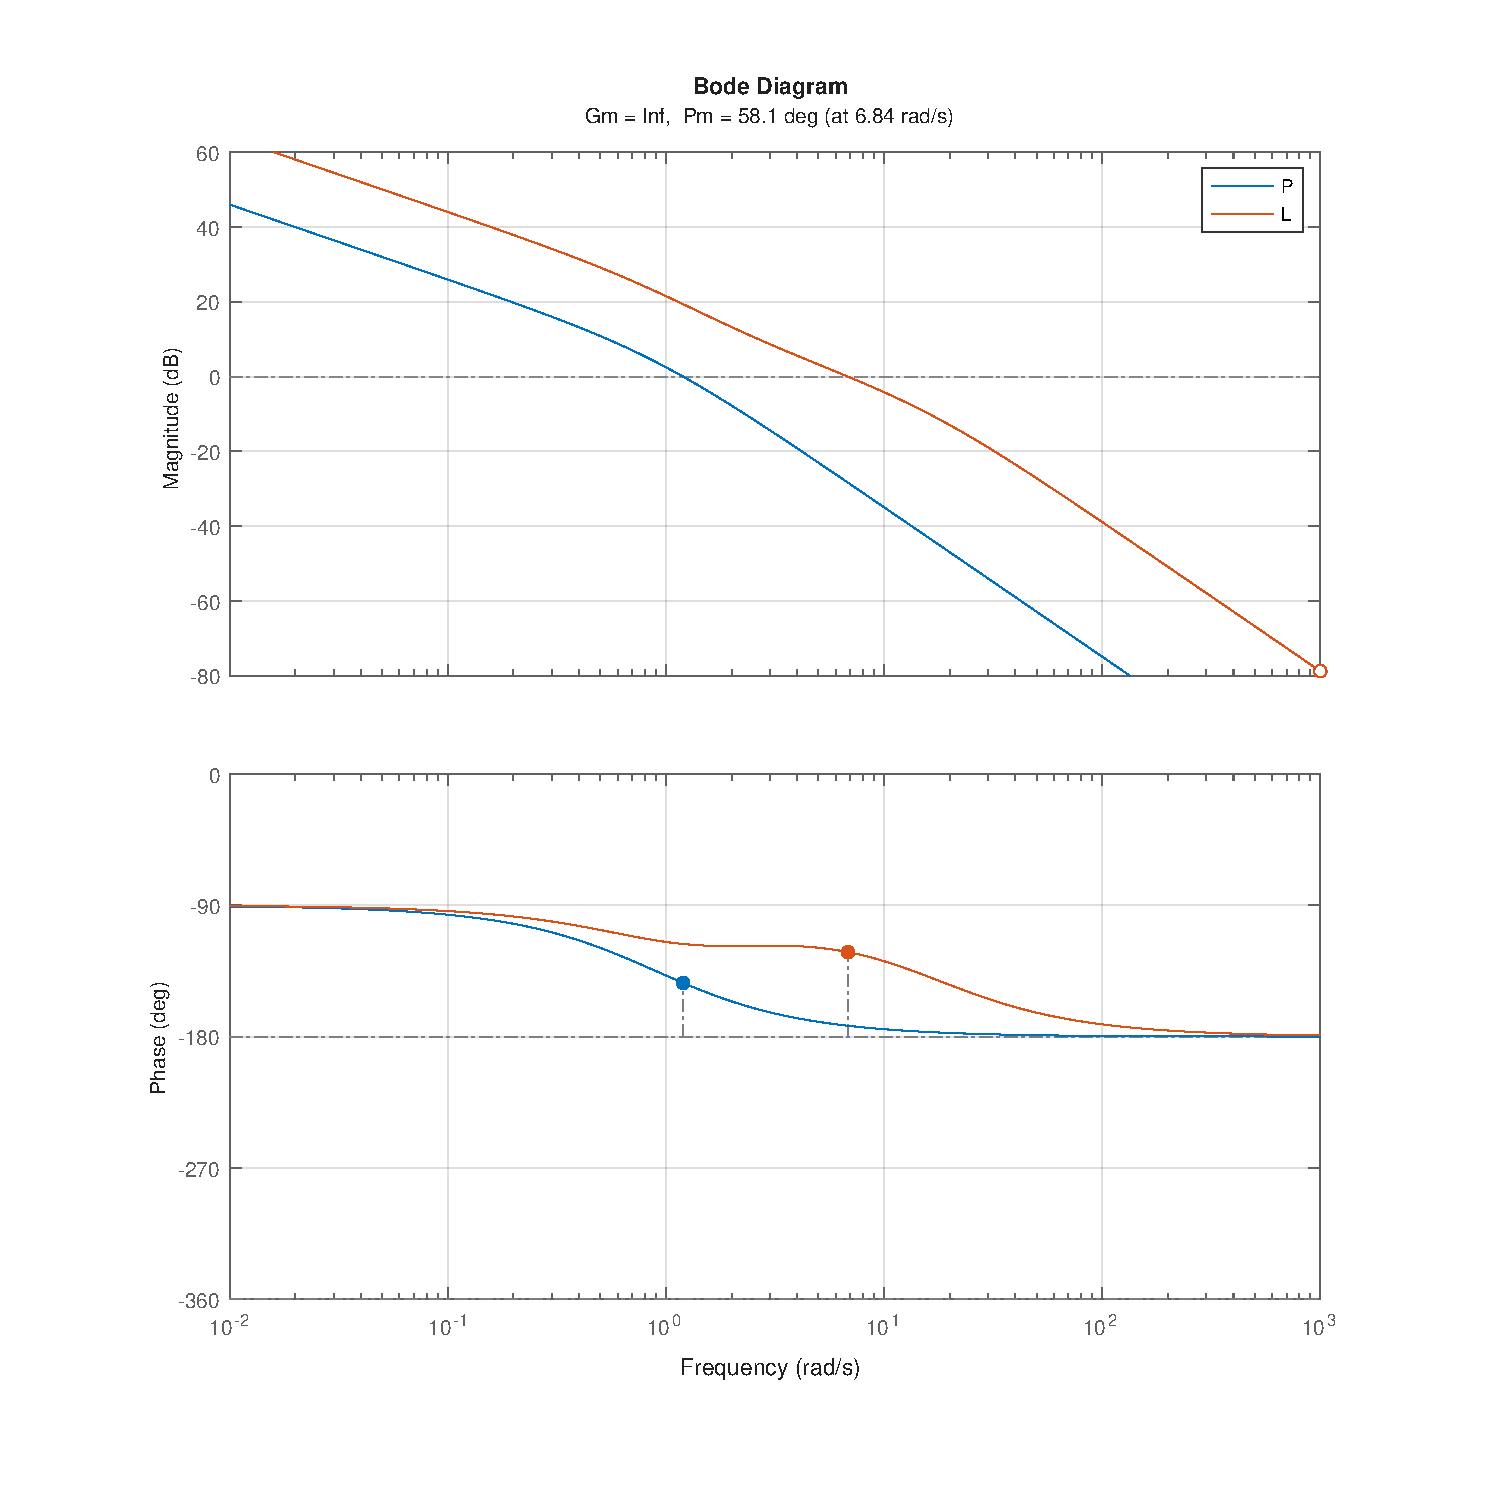
\includegraphics[width=0.5\linewidth]{fig_Parametrierung_Linienfolgeregler/Bode_Plot_Prozess_geregelt.pdf}
    \caption{Bodeplot mit eingezeichnter Phasen- und Amplitudenreserve des geregelten Prozesses}~\label{fig:MarginPlot_geregelt}
\end{figure}

\begin{figure}[H]
    \centering
    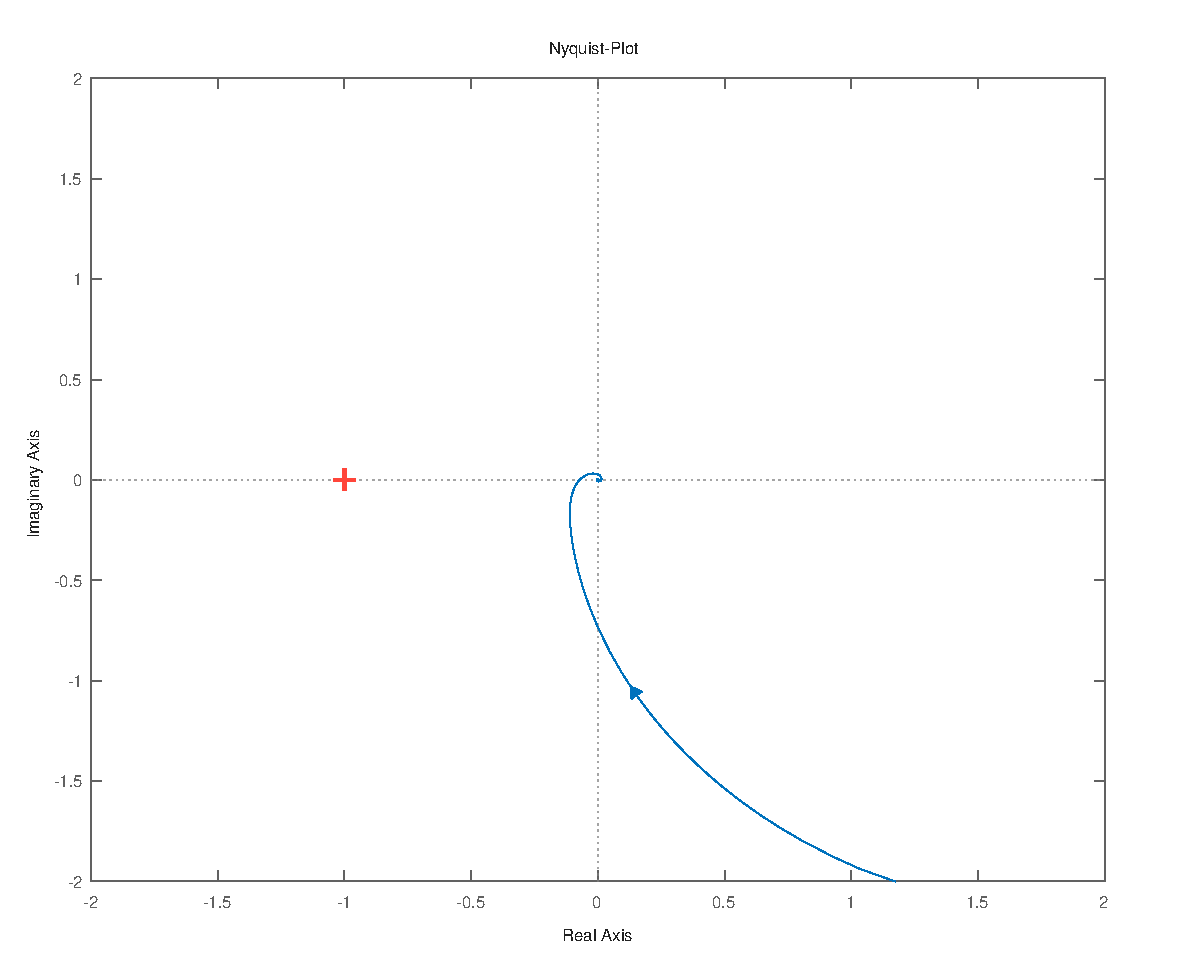
\includegraphics[width=0.5\linewidth]{fig_Parametrierung_Linienfolgeregler/NyquistPlot_System_geregelt.pdf}
    \caption{Nyquistdiagramm des geregelten Prozesses $P(s)$}~\label{fig:Nyquist_geregelt}
\end{figure}

\subsubsection*{Implementierung des Reglers in MotionController Firmware}

Mit Hilfe der \textit{Tustin-Approximation} kann der gefundene Regler
zeitdiskret approximiert werden. Es ergibt sich folgende Differenzengleichung
für den Regler $C(z)$.

\[
    u[k] = \beta \cdot e[k] - \beta \cdot e[k - 1] + \alpha \cdot u[k - 1]
\]

Der Regler verwendet die Parameter $\alpha = 0.2308$ und $\beta = 196.9$.

% TODO Regler C Zeitdiskretisieren und in Firmware testen
-> Abbildung bestätigung der Funktion darstellen. Dazu Test mit Firmware machen.

\end{document}